\refstepcounter{chapter}
\addcontentsline{toc}{chapter}{Maintenance}

\setsectiontitle{Important Notes}

\subsection*{Lubrication of the Machine}
\begin{itemize}
    \item Lubrication and cooling lubrication of the machine are summarized in the following pages of the operator's manual:
    \begin{itemize}
        \item 7.02-1 \textbf{Machine Lubrication Plan}
        \item 7.03-1 \textbf{Lubrication Regulations}
        \item 7.06-1 \textbf{Lubricant Recommendations}
        \item 7.07-1 \textbf{Coolants}
    \end{itemize}
    \item Lubrication and maintenance of additional equipment are described in Section 6 of the \\operator's manual, categorized by equipment.
    \item The designation of lubricants and their labeling in this manual comply with the new German standard DIN 51 502 (November 1979).
    \item The designation of liquid lubricants follows the ISO viscosity classification based on the kinematic viscosity at 40°C, as specified in DIN 51 519 (July 1976).
    \item The machine lubrication plan (7.02-1) and lubrication regulations (7.03-1) adhere to DIN 8659 (Draft, December 1978).
    \item \textbf{On the machine, oil lubrication nipples are marked in red, while grease nipples are marked with yellow identification discs.} Additionally, identification plates for lubrication nipples and filling points are attached in accordance with DIN 51 502.
\end{itemize}

\subsection*{Lubricants}
\begin{itemize}
    \item A key requirement for operational safety and machine longevity is the use of suitable \\lubricants.
    \item The machine is delivered pre-filled\footnotemark.
    \item The lubricants used for the initial filling (see 7.06-1) should be used continuously. If this is not possible for operational reasons, alternative products from the lubricant \\selection table (7.06-2 and 7.06-3) may be used.
\end{itemize}

\subsection*{Maintenance Tasks}
\begin{itemize}
    \item Apart from lubrication and cooling lubrication, all other maintenance tasks are summarized in 7.20-1 of the operator’s manual.
    \item Maintenance tasks must be performed diligently at the specified intervals.
    \item Maintenance intervals complement each other, meaning that if a 1000-hour task is due, the 40-hour tasks must also be completed. This applies to all other intervals.
    \item Section 9 of the operator's manual contains detailed disassembly instructions for major components.
\end{itemize}

\footnotetext{\textbf{Exception:} Lubrication oil for the drive wheel of the horizontal working spindle, see 1.09-1.}

\setsectiontitle{Machine Lubrication Plan}

\begin{figure}[H]
    \centering
    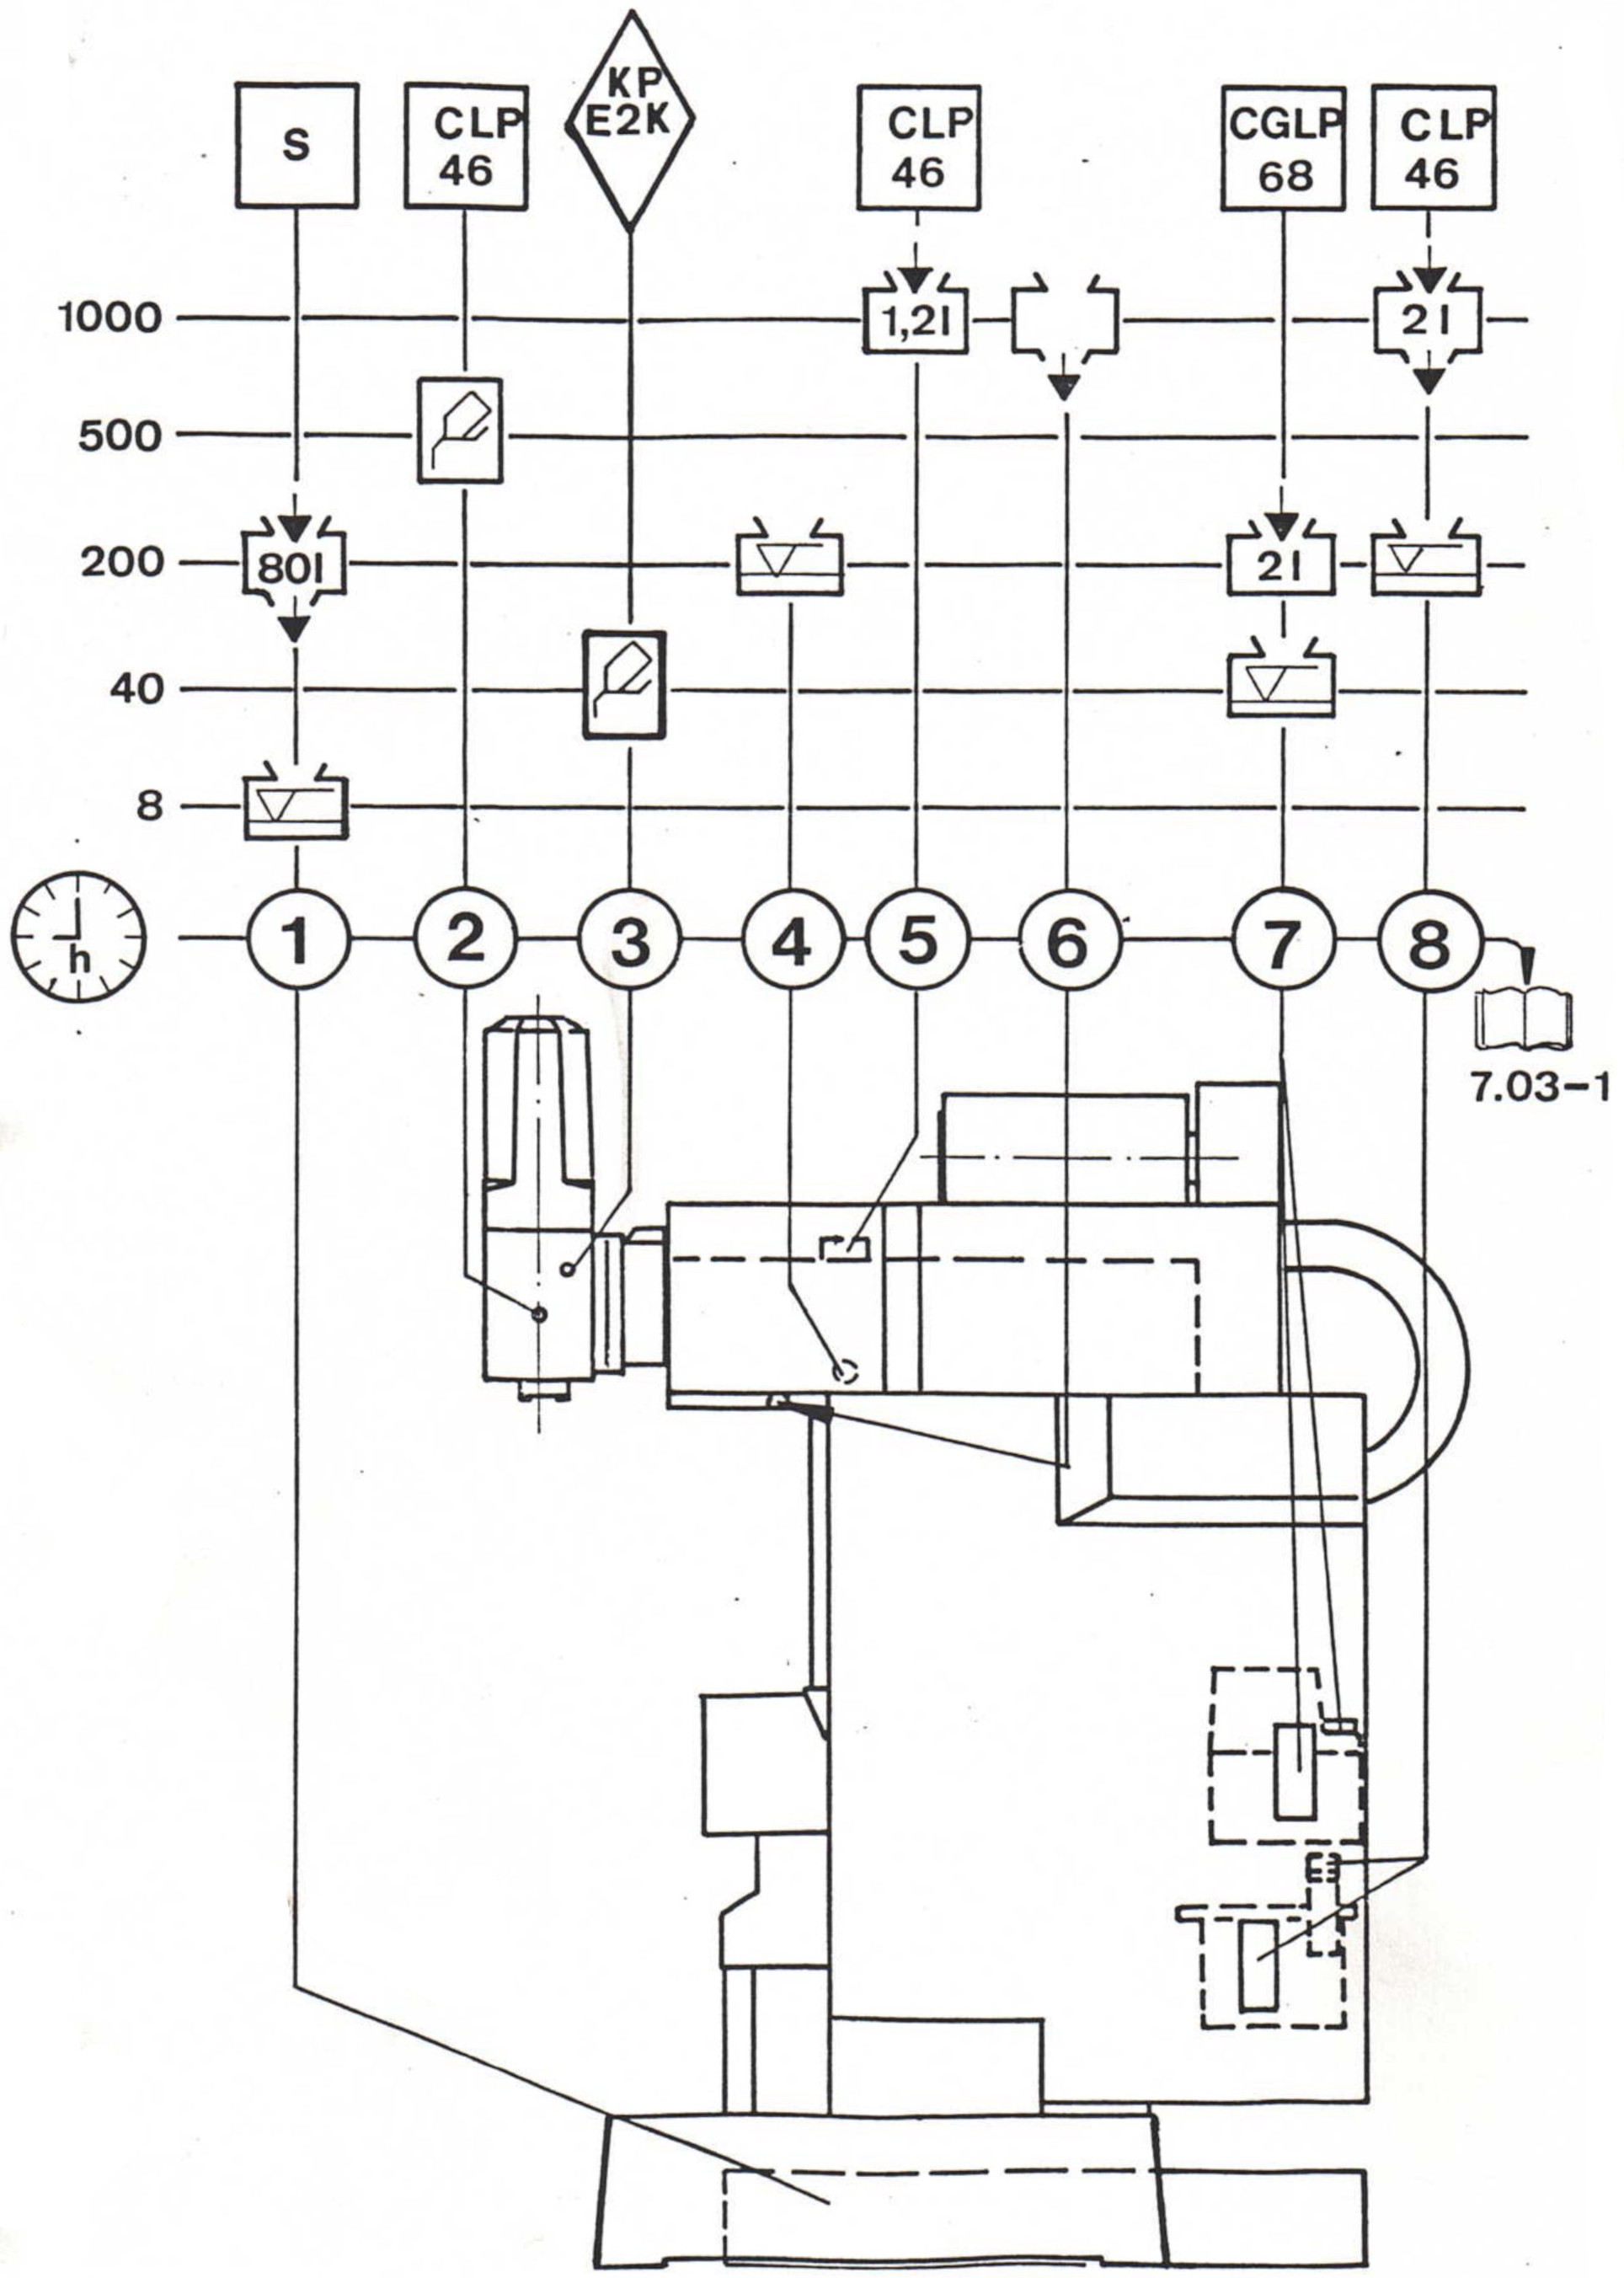
\includegraphics[width=0.9\textwidth]{chapter7/machine_lubrication_plan.jpg}
\end{figure}

\setsectiontitle{Lubrication Schedule}


\begin{table}[H]
    \centering
    \renewcommand{\arraystretch}{1.3}
    \begin{tabular}{|p{2cm}|p{1cm}|p{1.2cm}|p{7cm}|p{2cm}|p{2cm}|}
        \hline
        \hline
        \textbf{Interv. in Operating Hours} & \textbf{No. in Plan} & \textbf{Task Symbol} & \textbf{Task Description} & \textbf{Quantity} & \textbf{See Sheet} \\
        \hline
        \hline
        \multirow{1}{*}{8} & 1 & \raisebox{-\height}{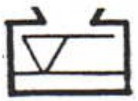
\includegraphics[width=10mm]{chapter7/coolant_level_check.jpg}} & Check coolant level in the coolant reservoir (keep as full as possible). & ---- & 3.22-1 \\
        \hline
        \multirow{2}{*}{40} & 3 \footnotemark[1] & \raisebox{-\height}{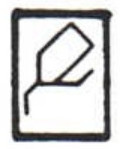
\includegraphics[width=10mm]{chapter7/lubrication.jpg}} & Lubricate bevel gear in the vertical milling head with Klüber-Isoflex NBU 15 (1 nipple, yellow marking). & 2-3 strokes & ---- \\
        \cline{2-6}
        & 7 & \raisebox{-\height}{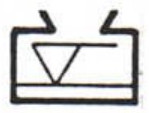
\includegraphics[width=10mm]{chapter7/oil_check.jpg}} & Check oil level in the central lubrication unit, refill if necessary. & ---- & 3.20-3 \\
        \hline
        \multirow{4}{*}{200} & 1 & \raisebox{-\height}{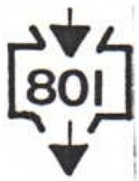
\includegraphics[width=10mm]{chapter7/coolant_change.jpg}} & Change coolant, clean tank. & approx. 80 l & 3.22-1, 7.07-4 \\
        \cline{2-6}
        & 4 & \raisebox{-\height}{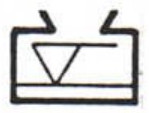
\includegraphics[width=10mm]{chapter7/oil_check.jpg}} & Check oil level for drive wheel, refill at position 5 if level drops below position 6. & ---- & ---- \\
        \cline{2-6}
        & 7 & \raisebox{-\height}{
\includegraphics[width=10mm]{chapter7/oil_fill.jpg}} & Refill oil into the central lubrication unit. & max. 2 l & 3.20-3 \\
        \cline{2-6}
        & 8 & \raisebox{-\height}{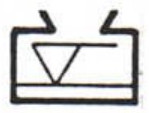
\includegraphics[width=10mm]{chapter7/oil_check.jpg}} & Check oil level in hydraulic unit. & ---- & 3.18-3 \\
        \hline
        \multirow{2}{*}{500} & 2 & \raisebox{-\height}{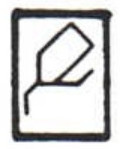
\includegraphics[width=10mm]{chapter7/lubrication.jpg}} & Lubricate quill in vertical milling head (1 nipple, red marking). & 2-3 strokes & ---- \\
        \hline
        \multirow{2}{*}{1000} & 5,6 & \raisebox{-\height}{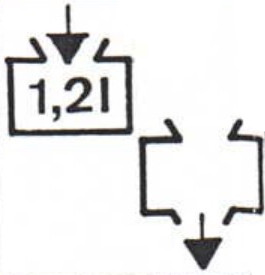
\includegraphics[width=13mm]{chapter7/oil_renew.jpg}} & Renew oil bath for drive wheel of horizontal spindle. & approx. 1,2 l & ---- \\
        \cline{2-6}
        & 8 & \raisebox{-\height}{
\includegraphics[width=10mm]{chapter7/oil_filter.jpg}} & Change hydraulic oil, clean filter. & max. 2 l & 3.18-3 \\
        \hline
        \hline
    \end{tabular}
\end{table}

\footnotetext[1]{For maximum load, e.g., continuous operation at maximum speed, lubricate every 8 operating hours!}

\setsectiontitle{Lubricant Recommendations}

\begin{table}[h]
    \centering
    \renewcommand{\arraystretch}{1.3}
    \begin{tabular}{|p{.75cm}|p{4cm}|p{2.7cm}|p{2.5cm}|p{4cm}|c|}
        \hline
        \hline
        \multicolumn{2}{|c|}{\textbf{Lubrication Point}} & \multicolumn{4}{c|}{\textbf{Lubricant Overview \footnotemark[1]}} \\
        \hline
        \hline
        \textbf{No. in Plan} & \textbf{Designation} & \textbf{Initial Fill Lubricant} & \textbf{Lubricant Type} & \textbf{Viscosity Range at 40°C / Analysis Data} & \textbf{Symbol} \\
        \hline
        \hline
        2 \newline 5 \newline 8 & Quill of the vertical milling head, Drive wheel of the horizontal work spindle, Hydraulic unit & Aral-Sumorol CM 46 (CMU) & Lubricating oil & CLP46/HLP46 41.4 - 50.6 & \raisebox{-\height}{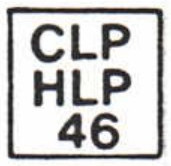
\includegraphics[height=8mm]{chapter7/clp_hlp_46.jpg}} \\
        \hline
        7 & Central lubrication unit, Universal built-in rotary table & Esso-Febis K 68 & Slideway oil & CGLP 68 (CG-HLP 68)/ 61.2 - 74.8 & \raisebox{-\height}{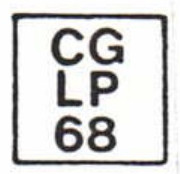
\includegraphics[height=8mm]{chapter7/cglp_68.jpg}} \\
        \hline
        3 & Bevel gear of the vertical milling head & Klüber-Iso-\newline flex \newline NBU 15 & Lubricating grease & KP E2K /\newline Walk penetration 265-295, Drip point approx. 180°C & \raisebox{-\height}{
\includegraphics[height=15mm]{chapter7/kp_e2k.jpg}} \\
        \hline
        1 & Cooling lubricant system & See Sheet 7.07-1 & Cooling lubricant & --- & \raisebox{-\height}{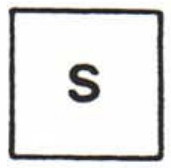
\includegraphics[height=8mm]{chapter7/s.jpg}} \\
        \hline
        \hline
    \end{tabular}
\end{table}

\footnotetext[1]{See Sheet 7.01-1 "Important Notes".}

\noindent Only the use of these lubricant types ensures the safe operation of the machine.  
We recommend continuing to use the initially filled lubricants, or if necessary, an equivalent type chosen based on operational requirements.

\notebox{WARNING}{\textbf{Liability cannot be accepted for the lubricants recommended in the following table.}}

Each of the lubricant manufacturers listed below maintains a lubrication service that can provide guidance and recommendations for all lubrication-related questions.

For intensive use of cooling lubricants, particularly in emulsion form the compatibility with the slideway oils used in the machine must be considered. See pages 7.07-1 to 7.07-3.

\setsectiontitle{Lubricant Selection Table}

\textcolor{RoyalBlue}{\textbf{Initial fill lubricants}} are highlighted in blue to indicate the factory-recommended oils. These should be used whenever possible to ensure proper machine function and longevity.

\renewcommand{\arraystretch}{1.3}
\begin{longtable}{|p{2.2cm}|p{2.7cm}|p{3cm}|p{3cm}|p{4.5cm}|}
    \hline
    \multicolumn{1}{|c|}{} & 
    \multicolumn{4}{c|}{\textbf{Lubricant Identification According to DIN 51 502}} \\
    \hline
    \textbf{Oil Type / Manufacturer} & 
    \raisebox{-\height}{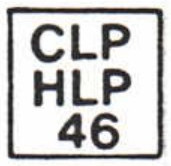
\includegraphics[height=15mm]{chapter7/clp_hlp_46.jpg}} & 
    \raisebox{-\height}{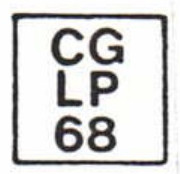
\includegraphics[height=15mm]{chapter7/cglp_68.jpg}} & 
    \raisebox{-\height}{
\includegraphics[height=15mm]{chapter7/kp_e2k.jpg}} & 
    \raisebox{-\height}{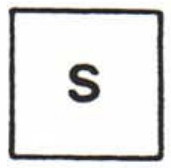
\includegraphics[height=15mm]{chapter7/s.jpg}} \newline \textbf{Cooling Lubricant} \\
    \hline
\endfirsthead

\hline
\multicolumn{1}{|c|}{} & 
\multicolumn{4}{c|}{\textbf{Lubricant Identification According to DIN 51 502}} \\
\hline
\textbf{Oil Type / Manufacturer} & 
\raisebox{-\height}{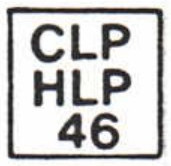
\includegraphics[height=15mm]{chapter7/clp_hlp_46.jpg}} & 
\raisebox{-\height}{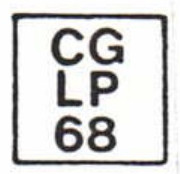
\includegraphics[height=15mm]{chapter7/cglp_68.jpg}} & 
\raisebox{-\height}{
\includegraphics[height=15mm]{chapter7/kp_e2k.jpg}} & 
\raisebox{-\height}{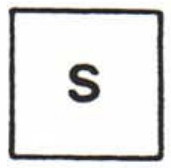
\includegraphics[height=15mm]{chapter7/s.jpg}} \newline \textbf{Cooling Lubricant} \\
\hline
\endhead
% Start of table body
    \hline
    ARAL & \textcolor{RoyalBlue}{\textbf{Sumorol CM 46}} & Aral-Deganit \newline BW 68 & --- & Sarol EP \newline Sarol 3965 \\
    \hline
    AVIA & AVILUB RL 46 \newline AVILUB HLPD 46 & AVILUB RSL 68-S & --- & AVILUB - Metacon ASBF \\
    \hline
    BP & Energol HL 46 \newline Energol HLP 46 & Maccurat 68 D & --- & (Cutora HX-Fedaro M) \\
    \hline
    Castrol & VARIO HDX \newline HYSPIN AWS 46 & MAGNA BDX 68 & --- & Clearedge EP 2840 \newline Hysol CB - Syntilo R \\
    \hline
    elf & POLYTELYS 46 \newline ELFOLNA 46 & MOGLIA 68 & --- & (Sarelf EP 34) \\
    \hline
    ESSO & NUTO H 46 \newline TERESSO 46 & \textcolor{RoyalBlue}{\textbf{FEBIS K 68}} & --- & Kutwell 30 \newline Kutwell 40 \\
    \hline
    FINA & FINA \newline HYDRAN CN 6 & ARTAC EP 68 & --- & (FINA VULSOL BST) \\
    \hline
    Fuchs & RENOLIN MR 15 & RENEP 2 & --- & RATAK DURANT 20 \newline RATAK TN 14/21 \\
    \hline
    Klüber & LAMORA 46 & LAMORA SUPER-POLADD 68 & \textcolor{RoyalBlue}{\textbf{Klüber Isoflex NBU 15}} & (ZELIOT-MS 250) \\
    \hline
    Mobil & D.T.E - Oil Medium \newline Mobil D.T.E 25 & BettbahnOil 68 & --- & Mobilmet 120 \newline Mobilmet 150 \newline EX 66/122 CF 1 \\
    \hline
    ÖMV & HTU 46 \newline HLP 46 & G 68 & --- & --- \\
    \hline
    Shell & Shell Tellus Oil C 46 \newline Shell Tellus Oil 46 & Tonna-Oil T 68 & --- & Shell-Dromus Oil BX \newline Shell-Dromus Oil EP \newline Shell-A 44 \\
    \hline
    TEXACO & Rando Oil 46 \newline HDB - 46 & Way Lubricant 68 & --- & Soluble Oil BS EP \newline Soluble Oil E \\
    \hline
    WISURA & Dynex 46 \newline Tempo 46 & BettbahnOil \newline 68 S (CGHLP 68) & --- & (Tralumat) \newline (WM 2998) \\
    \hline
    Zeller + Gmelin & GWA 2 ISO 46 \newline DHG 46 ISO & T 6 EP ISO 68 & --- & (Zubora 2000) \newline (Zubora 722 EP) \\
    \hline
\end{longtable}

\setsectiontitle{Coolant Lubricants\protect\footnotemark[1]}

For our milling machines and machining centers, only water-miscible and mineral-based coolant lubricants (in accordance with DIN 51385) should be used.

When selecting a coolant lubricant, care must be taken to ensure that the following undesirable properties \textbf{do not} occur:

\begin{enumerate}
    \item Adhesion and resinification of machine and control components, even if the coolant \\lubricant only enters in small quantities and cannot drain away.
    \item Incompatibility with the slideway oils used, which may cause them to decompose, harden, or be washed away.
    \item Corrosion protection must not decrease even after prolonged use of the coolant lubricant.
    \item Materials used in the machine for seals, wipers, etc. must not be attacked.
\end{enumerate}

\subsection*{Requirements for Coolant Lubricants\footnotemark[2]}

\begin{itemize}
    \item Good emulsifiability and stability even in harder water above 15° dH (5.4 m val).
    \item No damaging effects on machine components (metals, coatings, elastomers).
    \item Good lubricating properties and effectiveness for sliding machine elements.
    \item High resistance to decomposition and bacterial infestation.
    \item No harmful effects on humans.
    \item Toxicological test results and expert reports on skin compatibility should be available.
    \item No toxic additives such as nitrites or phenols.
    \item Must at least comply with the technical regulations for hazardous substances (TRgA 900).
    \item Used coolant lubricant emulsions must be separable by conventional separation processes.
\end{itemize}

\footnotetext[1]{DIN 51 385: 
\begin{minipage}[t]{\textwidth}
    \begin{itemize}
        \item Term 2.1 = Emulsifiable coolant lubricant (concentrate)
        \item Term 3.1 = Coolant lubricant emulsion (oil-in-water), ready-to-use mixture.
    \end{itemize}
    \vspace{.1cm}
\end{minipage}
}
\footnotetext[2]{See data sheet 7.07-2, 7.07-2.1.}

\setsectiontitle{Coolant Lubricants Data Sheet}

\setcounter{page}{2}

Selection criteria based on VKIS-Worksheet 3 - Sept. 83.

\subsection*{Physical and Chemical Reference Values}

\subsubsection*{6.1 Coolant Lubricant Concentrate}

\renewcommand{\arraystretch}{1.3}
\begin{longtable}{|p{6cm}|p{3cm}|p{3.5cm}|p{3.5cm}|}
    \hline
    \textbf{Property} & \textbf{Unit} & \textbf{Test Method} & \textbf{Reference Values} \\
    \hline
    \endfirsthead

    \hline
    \textbf{Property} & \textbf{Unit} & \textbf{Test Method} & \textbf{Reference Values} \\
    \hline
    \endhead

    \hline
    \endfoot

    \hline
    \endlastfoot

    Total mineral oil content & Vol. \% & DIN 51 417E & $> 35$ \\
    \hline
    Water content & Vol. \% & DIN 51 582 & Must be specified \\
    \hline
    Density & g/cm³ at 20°C & DIN 51 757 & 0.93 - 1.06 \\
    \hline
    Kinematic viscosity at 40°C & mm²/s (cSt) & DIN 51 366 & 20 - 120 \\
    \hline
    Kinematic viscosity at 20°C & mm²/s (cSt) & DIN 51 562 \newline DIN 53 015 & 50 - 300 \\
    \hline
    Refractive index & $n_D$ 20°C & DIN 51 423 & Must be specified \\
    \hline
    Flash point & + °C & DIN 51 376 & $> 130$ \\
    \hline
    Pour point & - °C & DIN 51 583 & 10 - 15 \\
    \hline
    EP additives (Mass. \%) & P \newline S \newline CI & DIN 51 363 \newline DIN 51 400 \newline DIN 51 577 & Must be specified \\
    \hline
    Sulfated ash (Mass. \%) &  & DIN 51 575 & --- \\
    \hline
    Preservatives & --- & --- & Type and amount must be specified \\
    \hline
    Silicones & \% & --- & Must be specified \\
    \hline
    Boron content & --- & --- & Must be specified \\
    \hline
    IR Spectrum & --- & --- & Must be specified \\
    \hline
\end{longtable}
\newpage

\subsubsection*{6.2 Water-Mixed Coolant Lubricant (Emulsion)}

\renewcommand{\arraystretch}{1.3}
\begin{longtable}{|p{6cm}|p{3cm}|p{2cm}|p{2.5cm}|p{2cm}|}
    \hline
    \textbf{Property} & \textbf{Concentration} & \textbf{Unit} & \textbf{Test Method} & \textbf{Reference} \newline \textbf{Values} \\
    \hline
    \endfirsthead

    \hline
    \textbf{Property} & \textbf{Concentration} & \textbf{Unit} & \textbf{Test Method} & \textbf{Reference} \newline \textbf{Values} \\
    \hline
    \endhead

    \hline
    \endfoot

    \hline
    \endlastfoot

    pH value at:\footnotemark[1] \newline NW12 (12°d.H.)\footnotemark[2] & 
    2\% \newline 10\% & 
    --- & 
    DIN 51 369 & 
    8 - 9.4 \\
    \hline
    Thermal conductivity & 5\% & kcal/mh°C & --- & $> 0.45$ \\
    \hline
\end{longtable}

\footnotetext[1]{\hangindent=1.8em The pH value is a measure of alkalinity. A pH of 7.0 is neutral (e.g., pure drinking water). Emulsions with a pH lower than 7.0 are considered \enquote{acidic} and provide poor corrosion protection. Higher pH values (up to 10.0) improve corrosion resistance. However, a pH greater than 9.4 can cause etching on sliding machine elements and skin irritation for operators.}
\footnotetext[2]{%
\hangindent=1.8em "NW12" refers to \enquote{normal water} with a hardness of 12° d.H. (4.3 mval.).  
\\ 100 d.H. means: 10g calcium oxide per 100 liters of water.  
\enquote{d.H.} is the abbreviation for \enquote{Deutsche Härte} (German hardness), for example:  

\begin{description}
    \item[\hspace{1.8em}Soft water:] less than 6° d.H. \footnotemark[5]
    \item[\hspace{1.8em}Moderately hard water:] 6 - 12° d.H.
    \item[\hspace{1.8em}Hard water:] more than 12° d.H.
\end{description}

\hspace{.3em} The hardness of tap water can be obtained from the local water utility.
}

\subsubsection*{Additional Physicochemical Reference Values}

Selection criteria based on VKIS-Worksheet 3 - Sept. 83.

\renewcommand{\arraystretch}{1.3}
\begin{longtable}{|p{5cm}|p{1.5cm}|p{3.5cm}|p{3cm}|p{2.5cm}|}
    \hline
    \textbf{Property} & \textbf{Concen-} \newline \textbf{tration} & \textbf{Unit} & \textbf{Test Method} & \textbf{Reference Values} \\
    \hline
    \endfirsthead

    \hline
    \textbf{Property} & \textbf{Concen-} \newline \textbf{tration} & \textbf{Unit} & \textbf{Test Method} & \textbf{Reference Values} \\
    \hline
    \endhead

    Electrical conductivity & 5\% & $\mu$S/cm & DIN 38 404 & Must be specified \\
    \hline
    Corrosion protection capacity & 5\% & --- & DIN 51 360/1 & RO, SO\footnotemark[3] \\
    \hline
    Corrosion degree & 5\% & --- & DIN 51 360/2 & 0 \\
    \hline
    Corrosion effect on copper\footnotemark[4] & 2.5\% & mg/dm³ & VKIS-Worksheet No. 7 \newline (DIN 51 759) & --- \\
    \hline
    Stability \newline (with 3g NaCl/1) & 5\% & --- & DIN 51 367 & $<$ 95\% \\
    \hline
    Foam behavior at NW 12 & 5\% & --- & --- & To be agreed upon with the manufacturer \\
    \hline
    Adhesion and residue behavior & 5\% & --- & VKIS-Worksheet No. 9 & Non-sticky, slightly soluble \\
    \hline
    Behavior against elastomers S2 according to DIN 53504\footnotemark[4] & --- & --- & --- & See Table~\ref{tab:elastomer_test} \\
    \hline
    Acid-decomposable components & 2\% \newline 10\% & Mass. \% & DIN 51 368 & Must be specified \\
    \hline
    EP-Effect & --- & --- & VKIS-Worksheet No. 6 & --- \\
    \hline
    Wear resistance according to Reichert & 5\% & N/cm² & --- & Must be specified \\
    \hline
\end{longtable}

\renewcommand{\arraystretch}{1.3}
\begin{longtable}{|p{5cm}|p{1.5cm}|p{5.5cm}|p{4cm}|}
    \caption{Elastomer Test Results} \label{tab:elastomer_test} \\
    \hline
    \textbf{Elastomer Material} & \textbf{Concen-} \newline \textbf{tration} & \textbf{Test Method} & \textbf{Result} \\
    \hline
    \endfirsthead

    \hline
    \textbf{Elastomer Material} & \textbf{Concen-} \newline \textbf{tration} & \textbf{Test Method} & \textbf{Result} \\
    \hline
    \endhead

    \hline
    \endfoot

    \hline
    \endlastfoot

    \multirow{2}{*}{SRE-WBR 28} & 2\% & VDA-Prüfblatt 521-01 \newline (DIN E 53 538) & +0.5\% Vol. Change \\
    & 10\% & --- & +0.15\% Shore-A Change \\
    \hline
    \multirow{2}{*}{CFW 88 NBR/101} & 2\% & --- & --- \\
    & 10\% & --- & --- \\
    \hline
\end{longtable}

\footnotetext[3]{RO = No rust; SO = No black spotting.}
\footnotetext[4]{Discoloration: None, Deposit formation: None, Copper ion content: Max. 50.}
\footnotetext[5]{\hangindent=1.8em International notation for water hardness is "mval." (Sum of all dissolved minerals). Conversion: $\frac{\text{dH}}{2.8}$}
